\documentclass[nobib]{tufte-handout}

\title{Lecture 8: Vertex covers, Hamilton cycles, independent sets $\cdot$ 1MA020}

\author[Vilhelm Agdur]{Vilhelm Agdur\thanks{\href{mailto:vilhelm.agdur@math.uu.se}{\nolinkurl{vilhelm.agdur@math.uu.se}}}}

\date{15 November 2023}


%\geometry{showframe} % display margins for debugging page layout

\usepackage{graphicx} % allow embedded images
  \setkeys{Gin}{width=\linewidth,totalheight=\textheight,keepaspectratio}
  \graphicspath{{graphics/}} % set of paths to search for images
\usepackage{amsmath}  % extended mathematics
\usepackage{booktabs} % book-quality tables
\usepackage{units}    % non-stacked fractions and better unit spacing
\usepackage{multicol} % multiple column layout facilities
\usepackage{lipsum}   % filler text
\usepackage{fancyvrb} % extended verbatim environments
  \fvset{fontsize=\normalsize}% default font size for fancy-verbatim environments

\usepackage{color,soul} % Highlights for text

% Standardize command font styles and environments
\newcommand{\doccmd}[1]{\texttt{\textbackslash#1}}% command name -- adds backslash automatically
\newcommand{\docopt}[1]{\ensuremath{\langle}\textrm{\textit{#1}}\ensuremath{\rangle}}% optional command argument
\newcommand{\docarg}[1]{\textrm{\textit{#1}}}% (required) command argument
\newcommand{\docenv}[1]{\textsf{#1}}% environment name
\newcommand{\docpkg}[1]{\texttt{#1}}% package name
\newcommand{\doccls}[1]{\texttt{#1}}% document class name
\newcommand{\docclsopt}[1]{\texttt{#1}}% document class option name
\newenvironment{docspec}{\begin{quote}\noindent}{\end{quote}}% command specification environment

\include{mathcommands.extratex}

\begin{document}

\maketitle% this prints the handout title, author, and date

\begin{abstract}
\noindent
We begin by continuing to pursue consequences of the Ford-Fulkerson theorem, proving König's theorem. Then we proceed to show Dirac's theorem on the existence of Hamilton cycles, and we finish with a discussion on independent sets, proving the Caro-Wei theorem.
\end{abstract}

\section{König's theorem}

In our last lecture, we proved the Ford-Fulkerson theorem relating minimum cuts and maximal flows, and used it to prove the Hall marriage theorem on matchings in bipartite graphs. We begin this lecture by proving another result we can derive from Ford-Fulkerson, namely König's theorem about vertex covers of bipartite graphs.

\begin{definition}
    Let $G$ be a finite simple graph. A \emph{vertex cover} of $G$ is a subset $S\subseteq V$ such that every edge has an endpoint in $S$. The \emph{covering number} of $G$, denoted $\beta(G)$, is the minimum size of any vertex cover of $G$.
\end{definition}

\begin{example}
    A star graph has covering number $1$, while a complete graph on $n$ vertices has covering number $n-1$. A cycle graph on $2n$ vertices has covering number $n$.
\end{example}

\begin{theorem}[König's theorem]
    Let $G$ be a bipartite graph. Then the maximum cardinality of a matching on $G$ equals $\beta(G)$, the minimum cardinality of a vertex cover of $G$.

    \begin{proof}
        Let $M$ be a maximal matching in $G$, and like in the proof of the marriage theorem, construct a flow network $G'$ from $G$. As we saw in the proof of that theorem, this matching $M$ corresponds to a maximal flow in $G'$ of value $\abs{M}$. By Ford-Fulkerson, this means there is a minimum cut $S, T$ on $G'$ of capacity $\abs{M}$.

        \begin{figure}
            \centering
            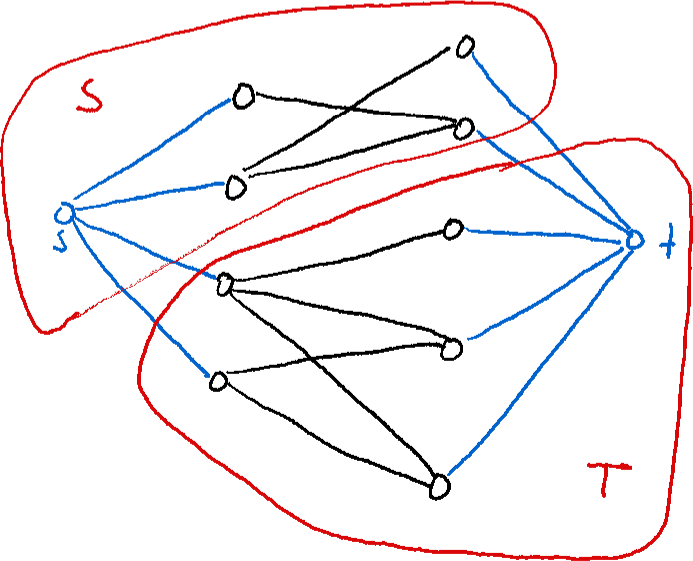
\includegraphics[width=0.5\textwidth]{graphics/L7_flows/bipartite_s_t_cut.png}
            \caption[][0cm]{A non-trivial minimal s-t-cut in a flow network created from a bipartite graph.}
            \label{fig:minimal_s_t_cut}
        \end{figure}

        Now, given this cut, let us construct a vertex cover. In particular, we let
        $$C = (A \cap T) \cup (B \cap S).$$
        That this $C$ is a vertex cover of $G$ is precisely the statement that there is no edge $a \to b$ with $a \in A \cap S$ and $b \in B \cap T$. This, however, is something we already saw is true for all minimum cuts in the previous proof -- because if there were such an edge, it would contribute $\infty$ to the capacity of the cut. So $C$ is indeed a vertex cover, and it is easy to convince oneself, looking at Figure \ref{fig:minimal_s_t_cut}, that $\abs{C} = c(S,T) = \abs{f} = \abs{M}$. So what we have seen is that the size of a maximal matching upper bounds the minimum vertex cover size, that is, $\beta(G) \leq \abs{M}$. 
        
        The other direction of the inequality in fact holds for all graphs, not just bipartite graphs -- every edge of a matching has to be covered by a vertex in the cover, and no vertex can cover more than one edge of the matching at a time. So any vertex cover has to have at least as many vertices in it as a maximal matching has edges.
    \end{proof}
\end{theorem}

\section{Hamilton cycles}

We studied, at the very beginning of the course, the notion of Eulerian circuits. The twin notion of Hamilton cycles appeared in our exercise session, but less us quickly repeat what we said about those.

\begin{definition}
    Let $G = (V,E)$ be a finite simple graph. A \emph{Hamilton cycle} in $G$ is a cycle that visits every vertex of $G$.\sidenote[][]{Recall that a \emph{cycle} by definition is a walk that starts and ends at the same vertex, and does not reuse any vertices other than the one it started with.} If $G$ admits a Hamilton cycle, we call it \emph{Hamiltonian}.
\end{definition}

Unlike for Eulerianity, there is no simple condition to determine whether a graph is Hamiltonian. In fact, computing whether a graph is Hamiltonian is an NP-Complete problem.

\begin{remark}
    Given a Hamiltonian cycle $C$ in $G$, we can easily construct a perfect matching of $G$ by just picking every second edge in the cycle. We can of course not in general turn a perfect matching into a Hamilton cycle, so Hamiltonicity is a stronger condition than having a perfect matching.
\end{remark}

That Hamiltonicity is an NP-Complete problem means we probably will never have any necessary and sufficient conditions for it. However, we can still prove results of the form ``if condition so-and-so holds, $G$ is Hamiltonian''. Let us prove the most famous such result.\sidenote[][]{It is named after a different Dirac than the one of quantum mechanics fame.}

\begin{theorem}[Dirac's theorem]
    Let $G = (V,E)$ be a simple graph on $n \geq 3$ vertices, such that every vertex has degree at least $\frac{n}{2}$. Then $G$ is Hamiltonian.

    \begin{proof}
        Assume $G$ is a graph satisfying the conditions of the theorem. Let us begin by observing that this $G$ cannot be disconnected -- if it were, the vertices in the smallest component would have fewer than half of the other vertices to connect to, so they would have too low degree.

        \begin{marginfigure}
            \centering
            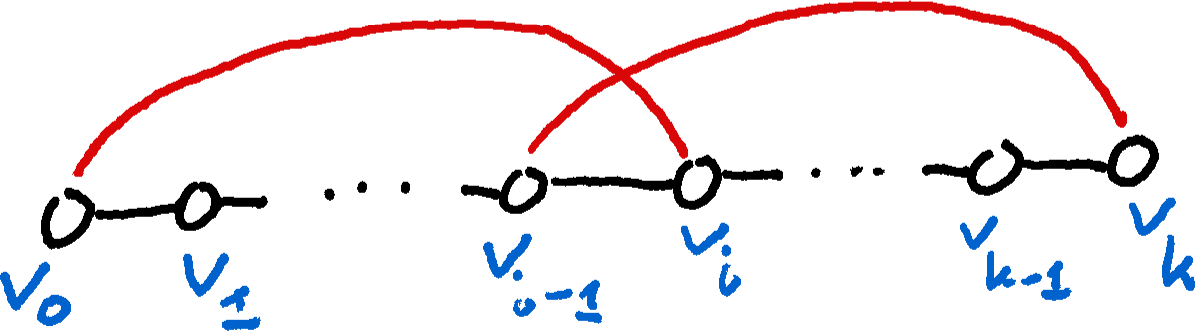
\includegraphics[width=1.0\textwidth]{graphics/L8_vx_covers_hamiltonicity_etc/diracs_thm_fig1.png}
            \caption{The path $P$ along with the configuration of two edges that must exist by the pigeonhole principle.}
            \label{fig:dirac_thm_fig1}
        \end{marginfigure}

        Now, consider a path $P$ of maximum length in $G$, say
        $$P = v_0\,e_1\,v_1\,\ldots\,v_{k-1}\,e_k\,v_k.$$
        Since this path is maximal, it contains all neighbours of $v_0$ and of $v_k$, since otherwise it could be extended. By our degree condition, there are (counting with multiplicity) at least $n$ such neighbours -- and so by essentially the pigeonhole principle, there must be an edge $e_i = \{v_{i-1},v_i\}$ on our path such that $v_i$ is a neighbour of $v_0$ and $v_{i-1}$ is a neighbour of $v_k$, as in Figure \ref{fig:dirac_thm_fig1}.

        Now we notice that this in fact lets us turn our path into a cycle -- we start at $v_0$, walk until $v_{i-1}$, then use the edge to $v_k$, walk backwards to $v_i$, and finally use the edge to $v_0$. This gives us a cycle $C$.

        \begin{marginfigure}
            \centering
            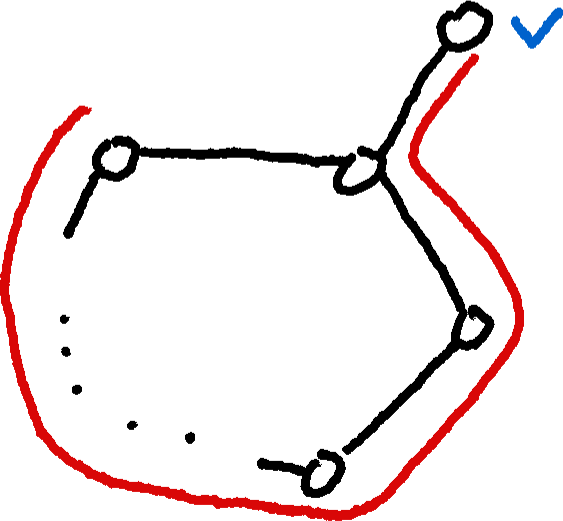
\includegraphics[width=0.6\textwidth]{graphics/L8_vx_covers_hamiltonicity_etc/diracs_thm_longer_path.png}
            \caption{A longer path than $P$ created from the cycle $C$, assuming it was not a Hamilton cycle.}
            \label{fig:diracs_thm_longer_path}
        \end{marginfigure}

        It remains to see that this $C$ is in fact a Hamilton cycle. So, suppose for contradiction that it is not, so that there is some vertex $v$ not on the cycle. Since $G$ is connected, we can in fact assume that this vertex is adjacent to some vertex of $C$. This, however, means we can create a longer path than $P$, by starting at $v$, walking onto $C$, and then following the cycle, as indicated in Figure \ref{fig:diracs_thm_longer_path}. However, we assumed $P$ was a maximal path, so we have a contradiction. So $C$ must be a Hamilton cycle.
    \end{proof}
\end{theorem}

\begin{figure}
    \centering
    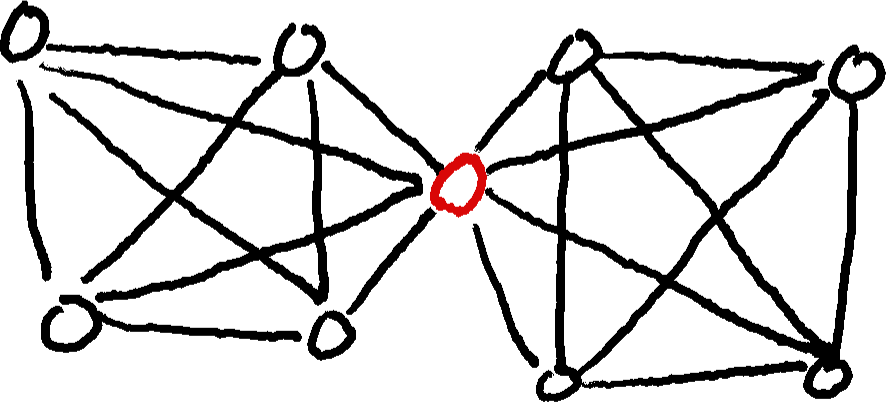
\includegraphics[width=0.65\textwidth]{graphics/L8_vx_covers_hamiltonicity_etc/diracs_theorem_counterexample.png}
    \caption[][0cm]{A graph used to show that the condition in Dirac's theorem is the best possible uniform lower bound.}
    \label{fig:dirac_counterexample}
  \end{figure}

\begin{remark}
    This result is in fact the best possible result with a uniform lower bound on the degrees of the vertices -- if we had picked any $k(n)$ less than $\frac{n}{2}$, there would be a counterexample. For example, consider the graph in Figure \ref{fig:dirac_counterexample}, where we have taken $k = \floor{\frac{n-1}{2}}$ and glued together two copies of $K_{k-1}$ by identifying two vertices. This graph has minimum degree $k$, but can of course not contain a Hamilton cycle since such a cycle would have to visit the glued-together vertex twice.
\end{remark}

Let us consider one particular example of a graph family that is Hamiltonian.

\begin{definition}
    The \emph{$d$-dimensional cube graph} has as its vertex set $\{0,1\}^d$, that is, the set of binary strings of length $d$. Two vertices are neighbours if the corresponding binary strings differ in only one position. The first few are illustrated in Figure \ref{fig:hypercubes}. 
\end{definition}

\begin{figure}
    \centering
    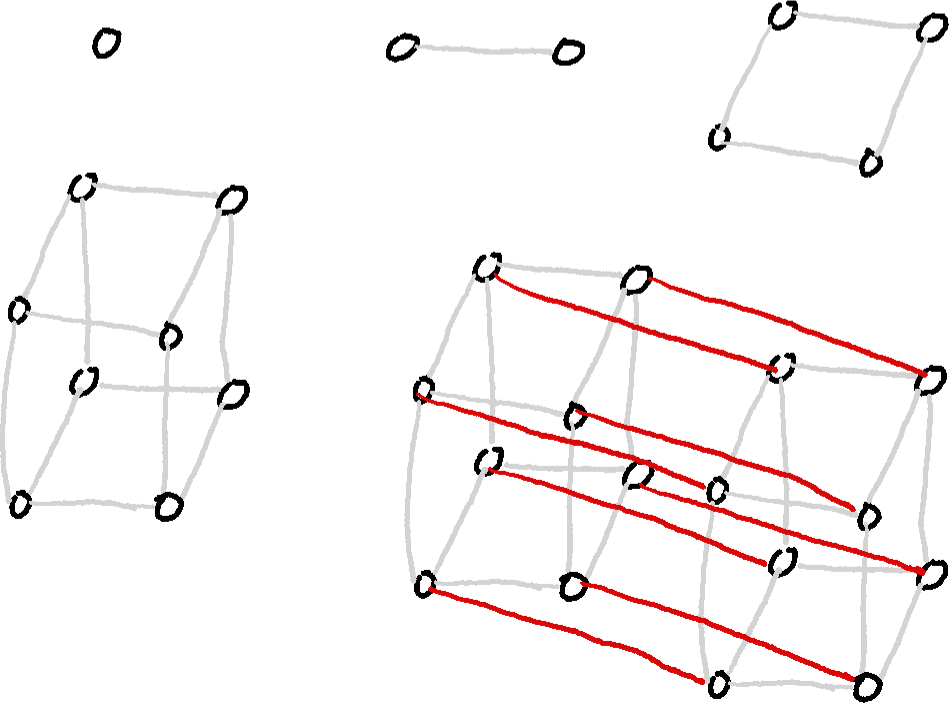
\includegraphics[width=0.65\textwidth]{graphics/L8_vx_covers_hamiltonicity_etc/binary_hypercubes.png}
    \caption[][0cm]{The $d$-dimensional cubes for $d = 0,1,2,4$. In the four-dimensional case we have highlighted some edges in red, to illustrate the inductive structure of the graph family.}
    \label{fig:hypercubes}
\end{figure}

\begin{theorem}\label{thm:hypercube_is_hamiltonian}
    The $d$-dimensional cube is Hamiltonian for all $d$.

    \begin{xca}
        Prove this.\qed
    \end{xca}
\end{theorem}

\begin{marginfigure}
    \centering
    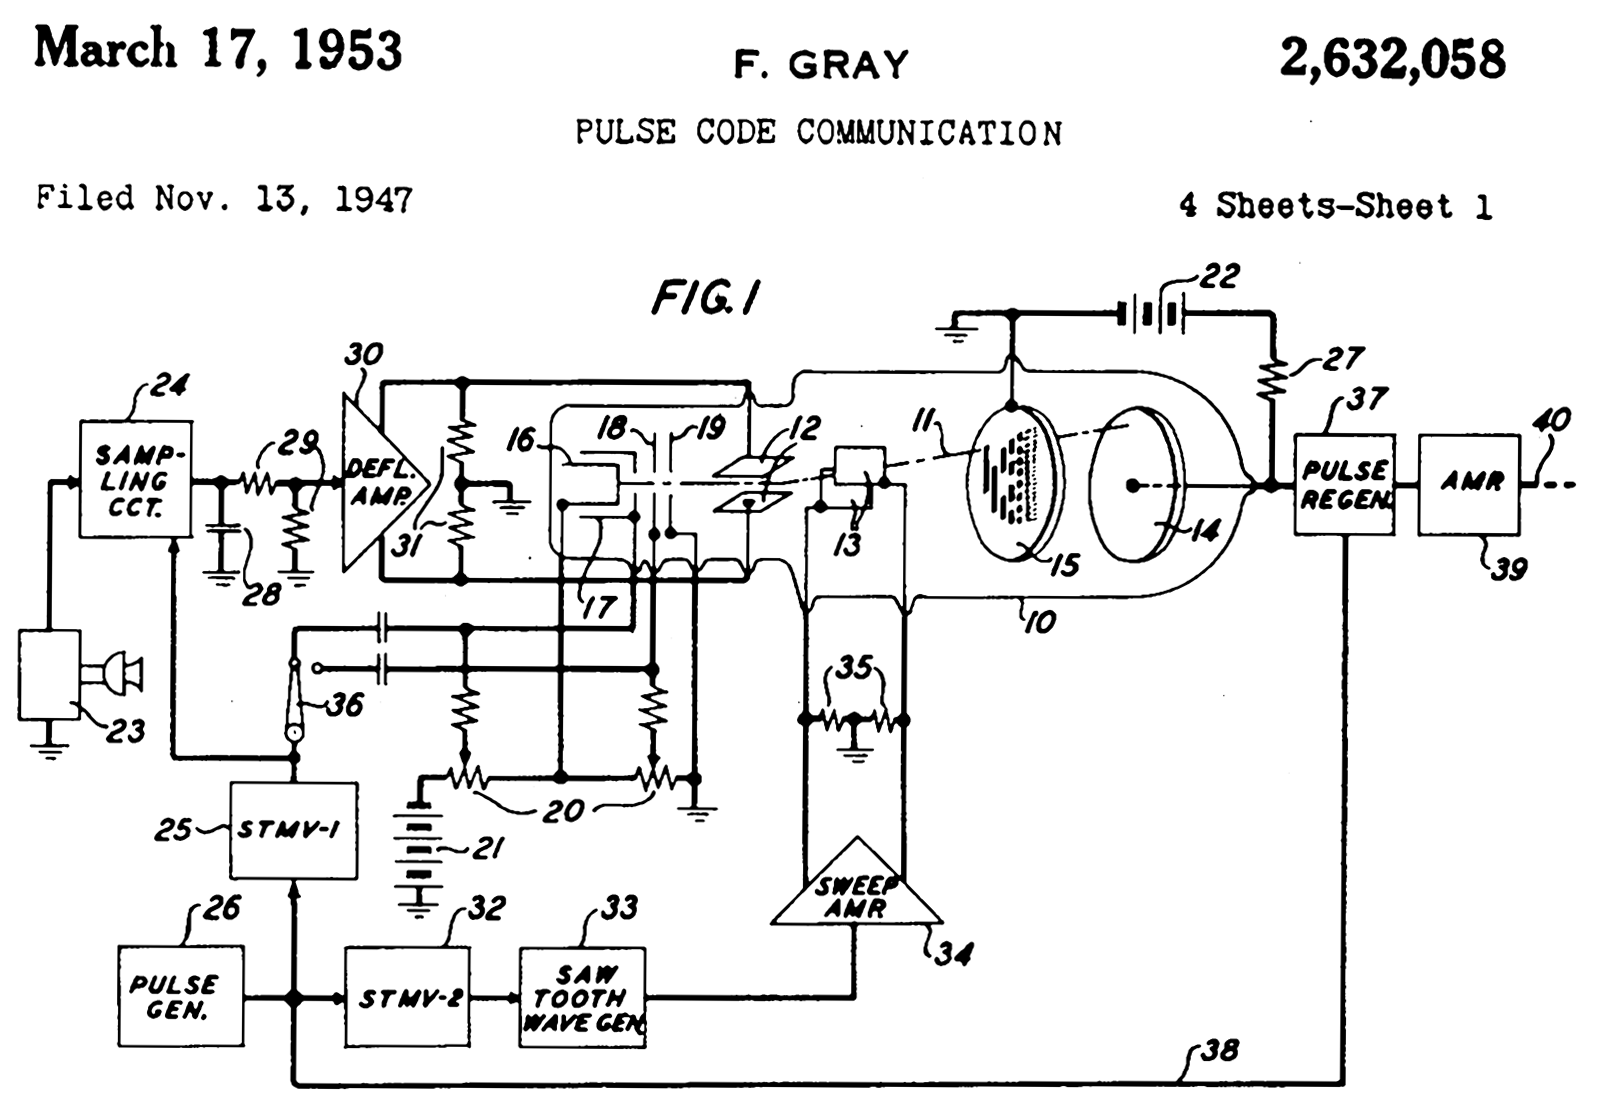
\includegraphics[width=1.0\textwidth]{graphics/L8_vx_covers_hamiltonicity_etc/gray_code_patent.png}
    \caption{The original patent for the device using a Gray code -- this supposedly happens in the thingy labelled by 15?}
    \label{fig:gray_code_patent}
\end{marginfigure}

\begin{remark}
    Notice that Theorem \ref{thm:hypercube_is_hamiltonian} gives us an ordering of the length-$d$ bit strings suh that going from one to the next always only requires us to change one of the bits. This ordering is known as the \emph{Gray code}, and it was originally invented to help in converting from analog to digital signals for colour television in the fifties.
\end{remark}

\section{Independent sets}

Another notion we encountered during the exercises is that of an \emph{independent set}. Let us repeat the definition again here.

\begin{definition}
    An \emph{independent set} in a graph $G = (V,E)$ is a subset $I \subseteq V$ of the vertices such that no two elements of $I$ are adjacent. The size of a maximum independent set in $G$ is called the \emph{independence number} of $G$, denoted $\alpha(G)$.
\end{definition}

We saw that this concept in fact connects to the concept of matchings if we consider the line graph of a graph.

\begin{definition}
    Given a graph $G = (V, E)$, the \emph{line graph} $L(G)$ of $G$ has as its vertices the \emph{edges} of $G$, and there is an edge between $e$ and $e'$ whenever they share an endpoint in $G$. This is illustrated in Figure \ref{fig:line_graph}.
\end{definition}

\begin{marginfigure}
    \centering
    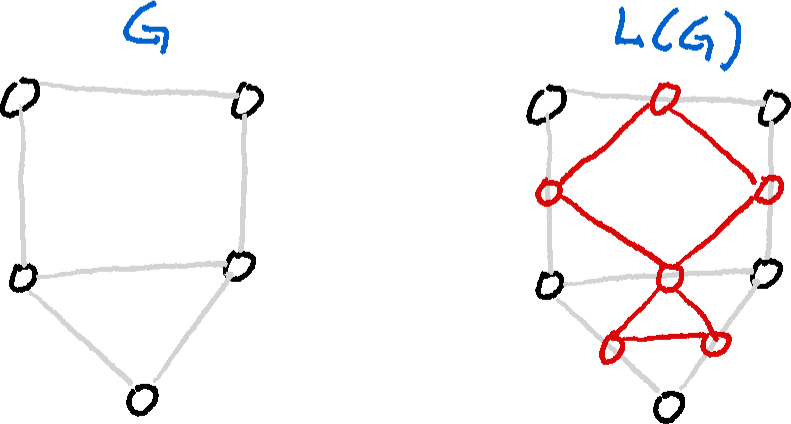
\includegraphics[width=0.85\textwidth]{graphics/L8_vx_covers_hamiltonicity_etc/line_graph.png}
    \caption{A graph $G$ on the left, and on the right we have its line graph $L(G)$ drawn on top of $G$ in red.}
    \label{fig:line_graph}
\end{marginfigure}

\begin{remark}
    A matching on a graph $G$ is precisely the same thing as an independent set in its line graph $L(G)$.
\end{remark}

In the exercises, we sketched out an argument as to why finding an independent set is NP-Complete. Let us now actually go through the details of the proof.

Our method will be to show that we can encode an instance of 3-SAT as a problem of finding an independent set of a certain size in a graph. This will prove that independent set is NP-Complete, because the Cook-Levin theorem tells us that 3-SAT is.

So first, let us define what an instance of 3-SAT is.

\begin{definition}
    An instance of 3-SAT is the problem of determining whether a given logical formula consisting of a conjunction of clauses of length $3$ is satisfiable. So, we have some set of logical variables $x_1, x_2, \ldots, x_n$. A literal is $x_i$ or $\notl x_i$ for some $i \in [n]$, and a clause of length $3$ is a disjunction of three literals, e.g. $x_4\vee \notl x_{10} \vee x_3$. We then take the conjunction of some number of such clauses, getting a formula like
    $$\left(x_1 \vee x_2 \vee \notl x_3\right) \wedge \left(x_2 \vee x_3 \vee \notl x_4\right) \wedge \left(x_1 \vee \notl x_2 \vee x_4\right),$$
    and what we want to determine is whether we can assign each variable a true or false value in such a way that the entire formula is true.
\end{definition}

\begin{theorem}
    The problem of determining whether a graph contains an independent set of size $k$ is NP-Complete.

    \begin{proof}
        We prove this by associating to each instance of 3-SAT an instance of the independent set problem, and showing that the 3-SAT formula is satisfiable if and only if there is an independent set of the right size in the graph.

        \begin{figure}
            \centering
            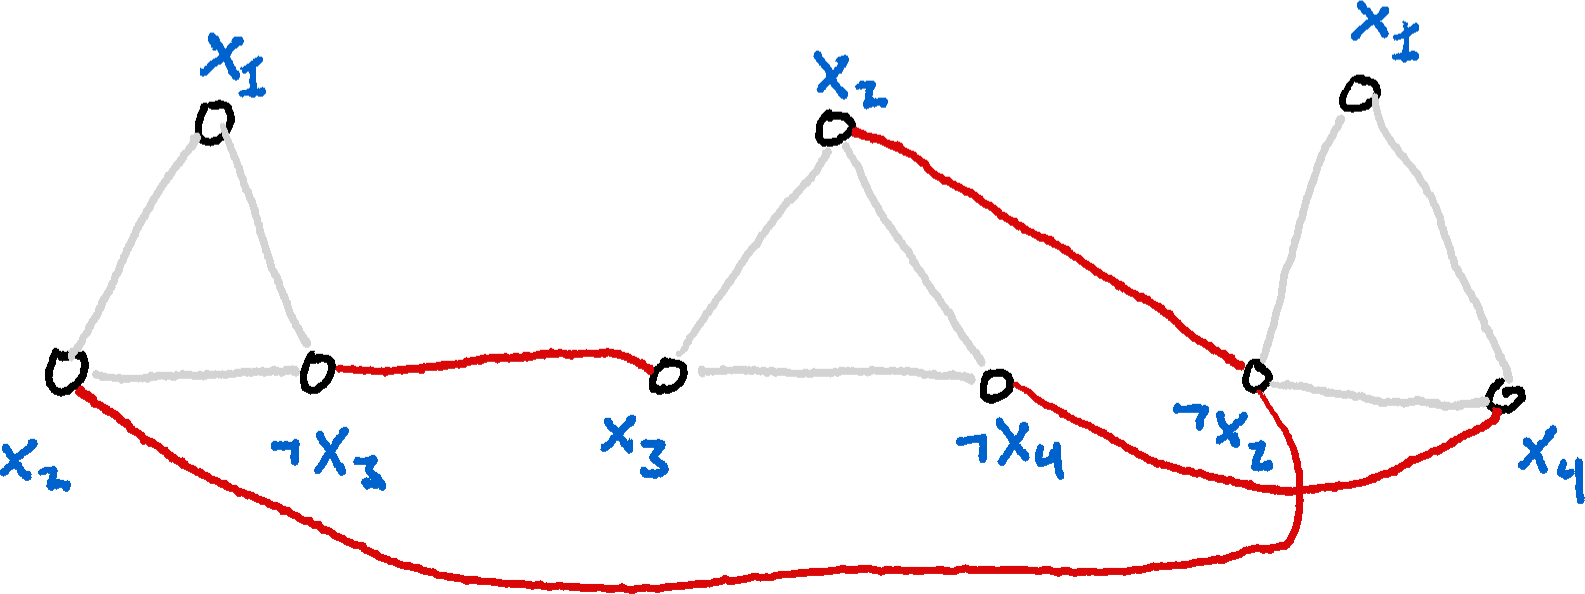
\includegraphics[width=0.65\textwidth]{graphics/L8_vx_covers_hamiltonicity_etc/3sat_triangles.png}
            \caption[][0cm]{The graph corresponding to the 3-SAT formula $\left(x_1 \vee x_2 \vee \notl x_3\right) \wedge \left(x_2 \vee x_3 \vee \notl x_4\right) \wedge \left(x_1 \vee \notl x_2 \vee x_4\right)$.}
            \label{fig:3sat_triangles}
        \end{figure}

        In particular, given a formula, we create a graph as follows: For each clause, draw a triangle, and label its vertices with the literals of the clause. Then, for each literal, draw an edge between its vertex and any vertex labelled with the negation of the literal. An example of this process is given in Figure \ref{fig:3sat_triangles}.

        We claim that this graph has an independent set of size equal to the number of clauses, i.e. the number of triangles we drew, if and only if the corresponding formula is satisfiable. If there is an independent set of that size, it is clear that it must contain one vertex from each triangle, which corresponds to picking one literal from each clause. Assigning the variables so that each of these literals becomes true gives a satisfying assignment.

        In the other direction, any satisfying assignment must of course make at least one literal per clause true. Picking a vertex corresponding to one of those literals from each clause gives us an independent set of the desired size.
    \end{proof}
\end{theorem}

\begin{remark}
    Earlier, we considered vertex covers, which are sets $S$ of vertices such that every edge has an endpoint in $S$. Notice that the complement of an independent set is a vertex cover -- if there were some edge that wasn't covered by this complement, both its endpoints would be in the complement of the complement, that is, in the independent set, which is of course impossible.

    So we have that the complement of a maximum independent set is a minimum vertex cover, and so $\alpha(G) + \beta(G) = n$. So we can use König's theorem also to find a maximum independent set in bipartite graphs.
\end{remark}

Similarly to how the NP-Completeness of finding Hamilton cycles meant we can't give a general characterization of those, we can't find an easy formula for $\alpha(G)$. We can, however, give some lower bounds on it -- and this will let us introduce a new proof technique to the course, the \emph{probabilistic method}.\sidenote[][]{As the name implies, this method requires some probability theory. It shouldn't involve anything much more involved than high school probability, and certainly nothing beyond an introductory university course in the subject.

This method features prominently in the course on combinatorics at this university, and the Caro-Wei theorem is proved in that course as well. That course gives more theoretical foundation to the probability theory, as well as applying the method to problems across combinatorics, not just to graph theory.}

\begin{theorem}[Caro-Wei]
    It holds for any graph $G = (V,E)$ that
    $$\alpha(G) \geq \sum_{v \in V} \frac{1}{d_v + 1}.$$

    \begin{proof}
        To prove this, we will consider a randomized greedy method of constructing an independent set, and show that it on average produces an independent set of this size.

        So, suppose we have been given a list $L$ of the vertices of $G$. Our greedy algorithm starts with a set $I = \emptyset$, and then at each time step it removes the first element $v$ of $L$, checks whether any neighbour of $v$ is in $I$, and if not, adds $v$ to $I$.
        
        That this process gives us an independent set is clear -- we never add in a vertex adjacent to something already in the set. Now, let us introduce the randomization to the algorithm, by picking a \emph{uniformly random} order for the list $L$.

        We can compute\sidenote[][]{This is a very standard computation in the probabilistic method, and one of the reasons it is so powerful -- we reduce a complicated calculation that involves the entire structure of a graph into a sum of easy calculations that just involve a vertex and its neighbours.} the expected size of the independent set found as
        $$\E{\abs{I}} = \E{\sum{v\in V} \ind{v \in I}} = \sum_{v \in V} \E{\ind{v \in V}} = \sum_{v\in V}\Prob{v \in I},$$
        so what we need is a lower bound on the probability that a given vertex is in the independent set.

        Now, clearly, if a vertex ends up first among all its neighbours on the list, then it will always be added to $I$, since none of its neighbours will be in $I$. So the probability that it ends up first on the list is a lower bound on the probability that it ends up in $I$.\sidenote[][]{
            \begin{xca}
                In general this is a lower bound, not an equality. Why?
            \end{xca}
        }

        The probability that it ends up on the list before all its neighbours is precisely the probability that in the list of just it and its neighbours, which has length $d_v + 1$, it ends up first. This probability is easily seen to be $\frac{1}{d_v + 1}$,\sidenote[][]{You can think of it as that we first choose a random slot for $v$, which can be done in $d_v + 1$ ways, and then place the rest of the elements. Only the choice of place for $v$ matters for the desired probability.} which gives us the desired lower bound of
        $$\E{\abs{I}} \geq \sum_{v\in V} \frac{1}{d_v + 1}.$$

        How do we get from this bound on the expected value to the statement that there actually exists such an independent set? We observe that the average outcome can't possibly be greater than every possible outcome, so there has to be an actual outcome which achieves this lower bound.
    \end{proof}
\end{theorem}

\section{Exercises}

\begin{xca}
    Show that the $d$-dimensional cube graph is bipartite.
\end{xca}


%\bibliography{references}
%\bibliographystyle{plainnat}

\end{document}
